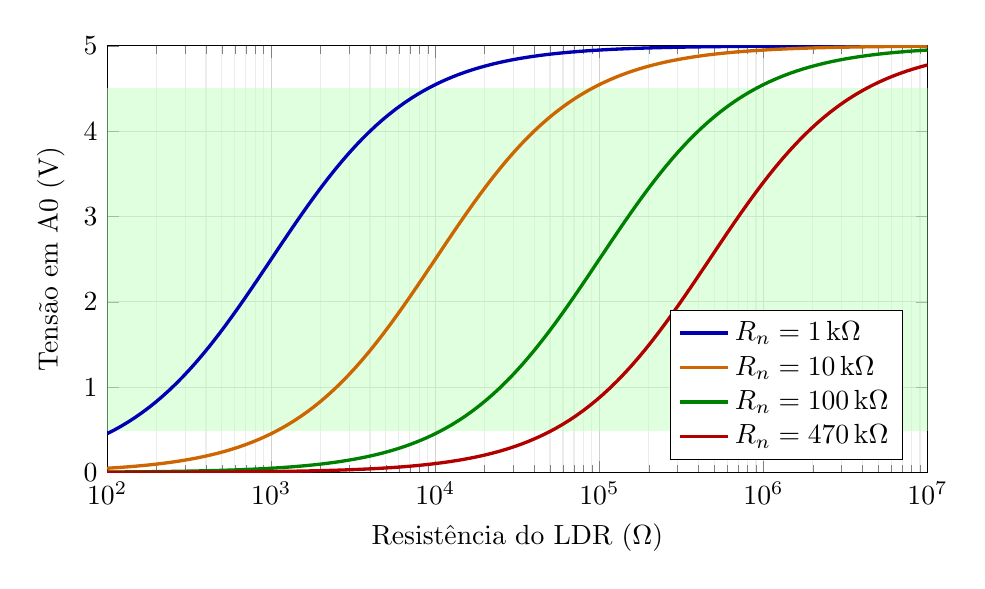
\begin{tikzpicture}
  \begin{semilogxaxis}[
    width=12cm, height=7cm,
    xmin=100, xmax=10000000, ymin=0, ymax=5,
    xlabel={Resistência do LDR ($\Omega$)},
    ylabel={Tensão em A0 (V)},
    grid=both, minor grid style={gray!15}, major grid style={gray!35},
    legend pos=south east, legend cell align=left,
  ]
    \addplot[fill=green!25, fill opacity=0.5, draw=none, forget plot] coordinates {(100,0.49) (10000000,0.49) (10000000,4.5) (100,4.5)} -- cycle;
    \addplot[domain=100:10000000, samples=120, very thick, blue!70!black] {5*x/(1000+x)};
    \addplot[domain=100:10000000, samples=120, very thick, orange!80!black] {5*x/(10000+x)};
    \addplot[domain=100:10000000, samples=120, very thick, green!50!black] {5*x/(100000+x)};
    \addplot[domain=100:10000000, samples=120, very thick, red!70!black] {5*x/(470000+x)};
    \legend{$R_n = 1\,\mathrm{k\Omega}$, $R_n = 10\,\mathrm{k\Omega}$, $R_n = 100\,\mathrm{k\Omega}$, $R_n = 470\,\mathrm{k\Omega}$}
  \end{semilogxaxis}
\end{tikzpicture}
